%%%
\usepackage[a4paper, total={6in, 8.6in}]{geometry}
%%
\usepackage{polyglossia}  \setdefaultlanguage{polish}
%%
\usepackage{booktabs}
\usepackage{fontspec}
\setmainfont{Cambria}
\setmathfont{Cambria Math}
%% Supress any other theorems (probably)
\newtheorem{theorem}{}
%%
%% This is not working
%% https://github.com/jgm/pandoc/issues/4384
%%
\makeatletter
\def\maxwidth{\ifdim\Gin@nat@width>\linewidth\linewidth\else\Gin@nat@width\fi}
\def\maxheight{\ifdim\Gin@nat@height>\textheight\textheight\else\Gin@nat@height\fi}
\renewcommand\section{\@startsection {section}{1}{\z@}%
                                   {-3.5ex \@plus -1ex \@minus -.2ex}%
                                   {2.3ex \@plus.2ex}%
                                   {\raggedright \normalfont\Large\bfseries}}
\renewcommand\subsection{\@startsection{subsection}{2}{\z@}%
                                     {-3.25ex\@plus -1ex \@minus -.2ex}%
                                     {1.5ex \@plus .2ex}%
                                     {\raggedright \normalfont\large\bfseries}}

\def\@makechapterhead#1{%
  %%\vspace*{50\p@}%
  {\parindent \z@ \raggedright \normalfont
    \ifnum \c@secnumdepth >\m@ne
      \if@mainmatter
        \large\bfseries \@chapapp\space \thechapter
        \par\nobreak
        %\vskip 5\p@
        %\medskip
      \fi
    \fi
    \interlinepenalty\@M
    \LARGE \bfseries #1\par\nobreak
    \vskip 20\p@
  }}
\def\@schapter#1{\if@twocolumn
                   \@topnewpage[\@makeschapterhead{#1}]%
                 \else
                   \@makeschapterhead{#1}%
                   \@afterheading
                 \fi}
\def\@makeschapterhead#1{%
  %%\vspace*{50\p@}%
  {\parindent \z@ \raggedright
    \normalfont
    \interlinepenalty\@M
    \huge \bfseries  #1\par\nobreak
    \vskip 20\p@
  }}


\makeatother
%%%
\AtBeginDocument{%%
 \let\maketitle\relax
  %% Insert title page
 \begin{titlepage}
 \begingroup  
 %% reset
 \setkeys{Gin}{width=210mm,height=300mm}
\vbox to \textheight{\vss%
   \hbox to\textwidth{\hss
     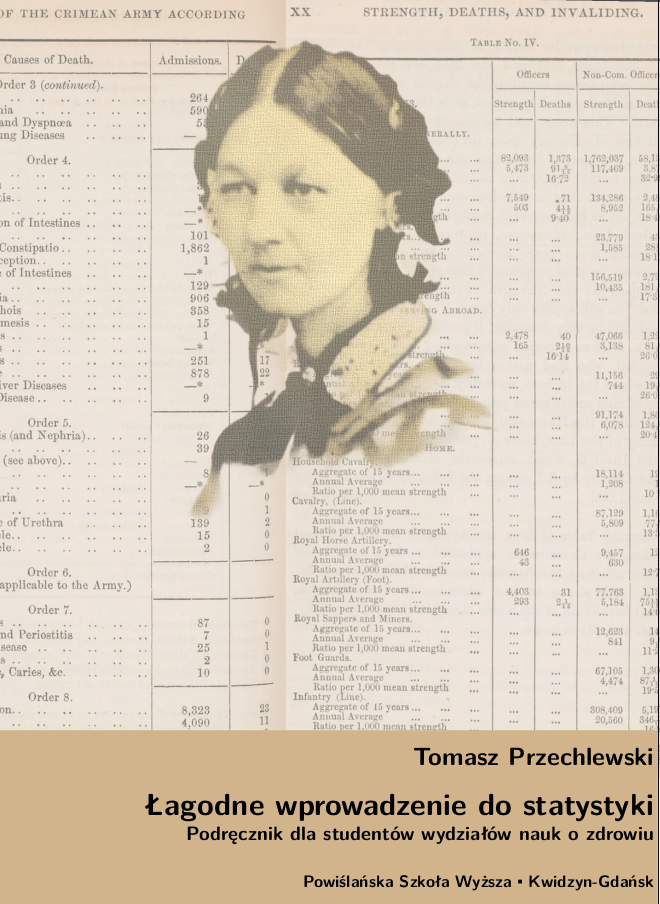
\includegraphics[width=210mm]{Cover_02.png}\hss}
   \vss}
\vbox to \textheight{\vskip20mm%
   Na okładce: Florence Nightingale i jej statystyki
  \vss
}
\endgroup
\end{titlepage}
\author{Tomasz Przechlewski\\ Powiślańska Szkoła Wyższa\\(Kwidzyn-Gdańsk)}%
}

\usepackage[most]{tcolorbox}
\newtcolorbox{TPexample}[1][]{%
    colback=black!5,
    colframe=black!5,
    notitle,
    sharp corners,
    enhanced,
    breakable,
}
\newenvironment{example}{\begin{TPexample}\parskip1ex}{\end{TPexample}}


\font\chineseFont="NotoSansTC-Regular" at 10pt
\def\chinese#1{{\chineseFont #1}}
\edef\bbChar{□}
\edef\bbCharX{☒}
\edef\bbArrowR{→}

\catcode`☒=\active
\catcode`□=\active
\catcode`→=\active
\def☒{\chinese{\bbCharX}} %% bb with X
\def□{\chinese{\bbChar}} %% ballot box
\def→{\chinese{\bbArrowR}} %% right arrow


\newenvironment{tof}{\begingroup\medskip }{\par\medskip\endgroup}
%%%
